\newpage
\section*{Szymon Chmiel}
 \subsection*{Wyrażenie matematyczne:}
Suma \textit{n} wyrazów ciągu geometrycznego:
  \[S_n = a_1 \frac{1 - q^n}{1 - q}\]
Suma \textit{n} wyrazów ciągu arytmetycznego:
  \[S_n = \frac{a_1 + a_2}{2} n\]

 \subsection*{Zdjęcie:}
 \begin{figure}[h]
     \centering
     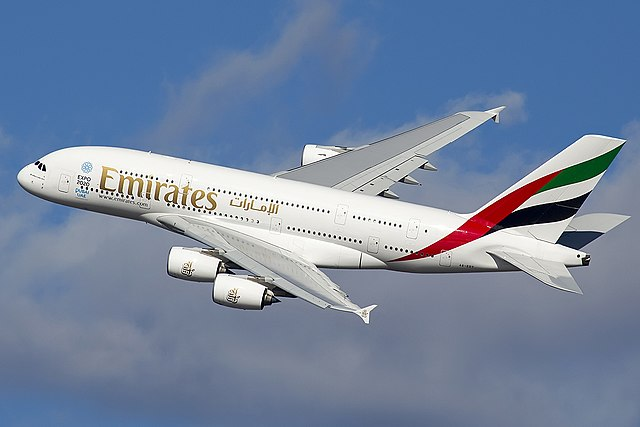
\includegraphics[width=0.75\textwidth]{pictures/samolot.jpg}
     \caption{Airbus A380}
     \label{fig:samolot}
 \end{figure}

 \subsection*{Tabela:}
 \begin{figure}[h]
     \centering
     \begin{center}
    \begin{tabular}{c|c|c|c}
         Samolot&Rozp. skrzydeł&Zasięg&Waga max.  \\
         \hline
         A380& 79.80 m&15 200 km&575 000 kg\\
         B747&68.50 m&14 815 km&442 250 kg\\
         A340&63.45 m&15 900 km& 380 000 kg\\
         B737&35.93 m&6500 km&82 600 kg\\
         A320&35.80 m&6300 km&79 000 kg
    \end{tabular}
\end{center}
     \caption{Zestawienie specyfikacji popularnych somolotów pasażerskich}
     \label{fig:enter-label}
 \end{figure}

 \subsection*{Linie Lotnicze:}
 \begin{itemize}
     \item Delta Airlines
     \item United Airlines
     \item Ryanair
     \item Emirates
     \item LOT
     \item KLM
     \item Pan American World Airways (do 1991)
 \end{itemize}
 \subsection*{Lotniska obsługujące największą ilość pasażerów:}
 \begin{enumerate}
     \item Atlanta, USA
     \item Dallas, USA
     \item Denver, USA
     \item Chicago, USA
     \item Dubai, ZEA
     \item Los Angeles, USA
     \item Istanbul, Turkey
     \item Heathrow - London, England
     \item Delhi, India
     \item Paris, France
 \end{enumerate}
 \subsection*{Największy samolot pasażerski świata}
 Zwany również latającym TIR-em, samolot A380 francuskiej firmy \textit{Airbus} nosi miano największego samolotu pasażerskiego świata(patrz Rysunek \ref{fig:samolot}). Przy podziale na 3 klasy może pomieścić do \textbf{560} pasażerów,  natomiast przy podziale na jedną klasę liczba ta wzrsta do niemal \textbf{900} pasażerów.

 Swój inauguracyjny lot komercyjny odbył \underline{15 października 2007} na trasie z Singapuru do Sydney. \\A380 jest również największym samolotem pasażerskim jeśli chodzi o rozpiętość skrzydeł, czy maksymalną masę startową(patrz Rysunek \ref{fig:enter-label})

 